\documentclass{../../theo-lecture/lecture}
\renewcommand{\thechapter}{\Alph{chapter}}
\begin{document}
    \chapter{Phänomenologie der Maxwell-Gleichungen}
    \section{Elektrisches Feld}
    Das Coulomb-Gesetz beschreibt die Kraft, die zwischen zwei Ladungen wirkt. Diese ist proportional zur Größe der beiden Ladungen sowie dem Quadrat des reziproken Abstands. Wir verwenden für die Vorlesung statt dem SI-System das Gauss-Einheitensystem, sodass der Proportionalitätsfaktor im Coulomb-Gesetz genau 1 wird.
    \section{Elektrische Feldstärke}
    Die Coulomb-Kraft ist die Kraft, die ein elektrisches Feld auf eine Ladung auswirkt. Mithilfe der Kraftmessung an einer Probeladung kann man also elektrische Felder messen. Analog beschreibt die Lorentz-Kraft die Kraft, die ein magnetisches Feld auf eine bewegte Ladung auswirkt, sodass man durch Kraftmessung an einer bewegten Probeladung magnetische Felder ebenfalls mit mechanischen Methoden messen kann. Das erklärt, warum man im Gauss-System keine eigene Einheit für die Ladung benötigt.
    \section{Maxwell-Gleichungen}
    Die Maxwell Gleichungen bilden die axiomatische Verbindung zwischen Feldern
    $\vec{E}, \vec{B}, \vec{D}, \vec{H}$ und den Ladungen $\rho, \vec{\jmath}$
    in Inertialsystemen (oder lokal in frei fallenden Systemen).
    \begin{enumerate}[(1)]
        \item Mithilfe der 1. Maxwell-Gleichung kann aus dem elektrischen Feld die Ladung bestimmt werden oder aus der Ladungsverteilung auf ein elektrisches Feld geschlossen werden.
        \begin{figure}[h]
            \centering
            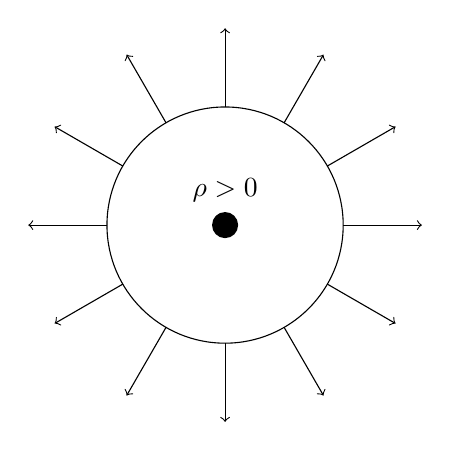
\begin{tikzpicture}
                \draw (0,0) circle (1.5cm);
                \node[fill = black, shape=circle, label=$\rho > 0$] (q) at (0,0) {}; 
                \foreach \a in {0,30,...,330} {\draw[->] (\a:1.5) -- (\a:2.5);}
            \end{tikzpicture}
            \caption{Die 1. Maxwell-Gleichung}
        \end{figure}
        Es folgt sofort aus dem Integralsatz von Gauss, dass das Volumenintegral über die Divergenz des elektrischen Felds gleich dem elektrischen Fluss durch die Oberfläche des betrachteten Volumens ist, was intuitiv sehr an das Verhalten einer Flüssigkeit erinnert. Die 1. Maxwell-Gleichung macht nun eine Aussage über die Größe der Divergenz bzw. des Flusses, dieser ist proportional zur Ladung im Inneren des Volumens.
        Setzen wir eine sphärische Symmetrie voraus, so folgt aus der Gleichung, dass das $\vec E$-Feld, das von einer Ladung ausgeht mit dem Abstand quadratisch abnimmt, sodass wir also das Coulomb-Gesetz in Beziehung zu den Maxwell-Gleichungen gesetzt haben.
        \item Die 2. Maxwell-Gleichung ist der ersten Gleichung sehr ähnlich. Die Größe des magnetischen Flusses durch eine geschlossene Fläche ist allerdings 0, da die Divergenz bereits 0 ist, was intuitiv bedeutet, dass es keine Quellen (also Ladungen) des magnetischen Felds gibt.
        \begin{figure}[ht]
            \centering
            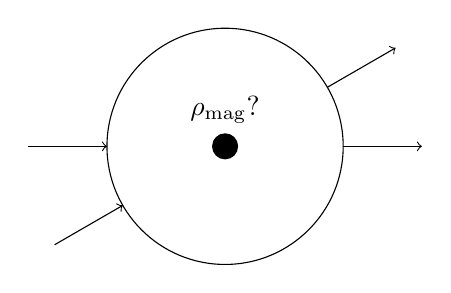
\begin{tikzpicture}
                \draw (0,0) circle (1.5cm);
                \node[fill=black,label=$\rho_{\mathrm{mag}}\text{?}$, shape=circle] (q) at (0,0) {};
                \draw[->] (-2.5, 0) -- (-1.5, 0);
                \draw[->] (210:2.5) -- (210:1.5);
                \draw[->] (1.5,0) -- (2.5,0);
                \draw[->] (30:1.5) -- (30:2.5);
            \end{tikzpicture}
            \caption{Die 2. Maxwell-Gleichung}
        \end{figure}
        Dass es keine magnetischen Ladungen geben muss, ist nicht klar, es wurden bisher einfach noch keine gefunden. Wie wir später sehen werden, wäre es kein Problem, eigentlich sogar sehr viel symmetrischer, wenn es magnetische Ladungen tatsächlich geben würde.
        \item Die 3. Maxwell-Gleichung ist auch bekannt als Induktionsgesetz von Faraday und stellt eine Verbindung her zwischen magnetischem Fluss durch eine Fläche und induzierter Spannung auf dem Rand der Fläche. Das $-$ auf der rechten Seite führt zur Lenz-Regel.
        \begin{figure}[ht]
            \centering
            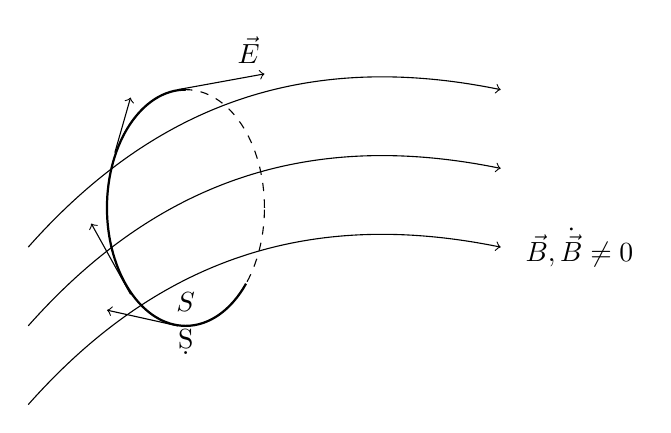
\begin{tikzpicture}
                \foreach \x in {0,1,2} {\draw[->] (0,\x) to[bend left] (6,\x+2);}
                \node (B) at (7,2) {$\vec B, \dot{ \vec{B}} \neq 0$};
                \draw[dashed] (2,2.5) ellipse (1 and 1.5);
                \draw[thick] (2,4) arc (90:320:1 and 1.5);
                \draw[->] (1.9,4) -- (3,4.2);
                \draw[->] (1.1,3.2) -- (1.3,3.9);
                \draw[->] (1.3, 1.4) -- (0.8, 2.3);
                \draw[->] (1.9,1) -- (1, 1.2);
                \node (E) at (2.8,4.5) {$\vec E$};
                \node (S) at (2,1.3) {$S$};
                \node (dS) at (2,.8) {$\d{S}$};
            \end{tikzpicture}
            \caption{Die 3. Maxwell-Gleichung}
        \end{figure}
        \item Die 4. Maxwell-Gleichung ist auch bekannt als Ampere-Gesetz und stellt eine Verbindung her zwischen elektrischen Fluss oder sich änderndem $\vec E$-Feld und einem magnetischen Feld auf dem Rand der Fläche. 
        \begin{figure}[ht]
            \centering
            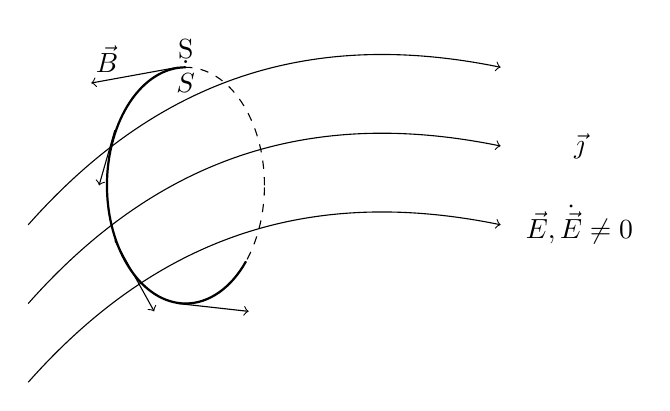
\begin{tikzpicture}
                \foreach \x in {0,1,2} {\draw[->] (0,\x) to[bend left] (6,\x+2);}
                \node (E) at (7,2) {$\vec E, \dot{\vec{E}} \neq 0$};
                \node (j) at (7, 3) {$\vec \jmath$};
                \draw[dashed] (2,2.5) ellipse (1 and 1.5);
                \draw[thick] (2,4) arc (90:320:1 and 1.5);
                \draw[->] (1.9,4) -- (.8,3.8);
                \draw[->] (1.1,3.2) -- (.9,2.5);
                \draw[->] (1.1, 1.8) -- (1.6, .9);
                \draw[->] (1.9,1) -- (2.8, .9);
                \node (B) at (1,4.1) {$\vec B$};
                \node (S) at (2,3.8) {$S$};
                \node (dS) at (2,4.2) {$\d{S}$};
            \end{tikzpicture}
            \caption{Die 4. Maxwell-Gleichung}
        \end{figure}
        Setzen wir zylindrische Symmetrie voraus, so erhalten wir, dass das $B$-Feld mit dem reziproken Abstand vom Strom abnimmt.
    \end{enumerate}
    \section{Eigenschaften der Maxwell-Gleichungen}
    \begin{itemize}
        \item Die Maxwell-Gleichungen sind lineare, partielle, hyperbolische Differenzialgleichungen (wird später noch erklärt).
        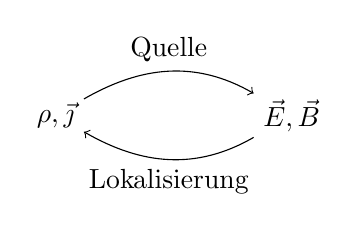
\begin{tikzpicture}
            \node (q) at (0,0) {$\rho, \vec \jmath$};
            \node (E) at (3,0) {$\vec E, \vec B$};
            \draw[->] (q) to[out = 30, in=150] node[above] {Quelle} (E);
            \draw[->] (E) to[out = -150, in=-30] node[below] {Lokalisierung} (q);
        \end{tikzpicture}
        \item Die Maxwell-Gleichungen ergeben nur Sinn in einem Bezugssystem, wir legen also ein Inertialsystem fest.
        \item Wir haben 2 $\div$-Gleichungen und 2 $\rot$-Gleichungen, also effektiv $1 + 1 + 3 + 3 = 8$ Gleichungen, wir untersuchen aber nur die Dynamik von $\vec E$- und $\vec B$-Feld ($3 + 3 = 6$ Komponenten). Sind die Maxwell-Gleichungen daher überbestimmt?
    \end{itemize}
    \section{Erhaltung der elektrischen Ladung}
    Aus der 1. und 4. Maxwell-Gleichung ergibt sich die sogenannte Kontinuitätsgleichung.
    Diese besagt, dass Ladungsänderung in einem Volumen gleich der elektrischen Stromdichte durch die Oberfläche ist.
    Die Elektrodynamik ist eine Kontinuumstheorie. Ladung ist dabei eine Art ,,Fluid``.
    \section{Elektromagnetische Dualität}
    Betrachtet man die Maxwell-Gleichungen im Vakuum, d.h. $\rho = 0$, $\vec{\jmath} = 0$, so kann man $\vec E \to \vec B,\quad \vec B \to -\vec E$ vertauschen, ohne dass sich an den Maxwell-Gleichungen etwas ändert (Dualität).
    Warum existieren eigentlich keine magnetischen Ladungen? Ergänzt man die Maxwell-Gleichungen auf symmetrische Weise um entsprechende Ausdrücke für die magnetische Ladung, so erhält man wieder eine Kontinuitätsgleichung für die magnetische Ladung.
    Die Maxwell-Gleichungen bestimmen also nicht nur die Dynamik von $\vec E$ und $\vec B$ Feldern, sondern auch die Erhaltung elektrischer und magnetischer Ladung und sind daher nicht überbestimmt.
    \section{Elektrodynamik in Materie}
    Elektrodynamik in Materie ist im Allgemeinen sehr kompliziert.
    Im einfachsten Fall ist die Wirkung linear, isotrop und instantan.
    Dann existiert eine effektive Beschreibung mithilfe von nur zwei Konstanten, nämlich der Dieelektrizitätskonstanten $e$ und der Permeabilitätskonstanten $\mu$.
    \section{elektrostatisches Potenzial}
    Dabei bedeutet elektrostatisch, dass alle Zeitableitungen 0 sind.
    \begin{figure}[h]
        \centering
        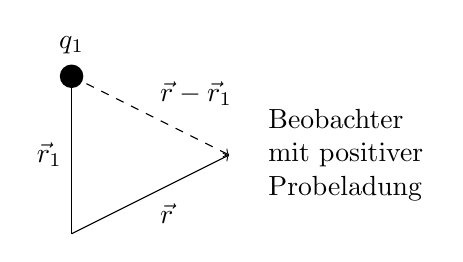
\begin{tikzpicture}
            \node[fill = black, shape = circle, inner sep = 3pt, label = $q_1$] (q1) at (0,2) {};
            \draw[->] (0,0) -- node[pos=.5, left] {$\vec r_1$} (0,2);
            \draw[->] (0,0) -- node[pos=.5, below right] {$\vec r$} (2,1);
            \draw[dashed, ->] (0,2) -- node[pos=.5, above right]{$\vec r - \vec r_1$} (2,1);
            \node[text width = 2cm] (beobachter) at (3.5,1) {Beobachter mit positiver Probeladung};
        \end{tikzpicture}
        \caption{Elektrisches Feld}
        \label{efeld}
    \end{figure}
    Für das elektrische Feld aus Abbildung~\ref{efeld} gilt daher einfach das Coulomb-Gesetz. 
    Bei vielen felderzeugenden Ladungen berechnen wir einfach die Superposition der einzelnen Felder.
    Da es sich bei der Elektrodynamik um eine Kontinuumstheorie handelt, gehen wir von diskreten Ladungen $q$ zu einer kontinuierlichen Ladungsverteilung $\rho$ über und erhalten eine kontinuierliche Version des Coulomb-Gesetzes.
    Dadurch sind wir in der Ladung, ein elektrostatisches Potenzial zu definieren, sodass wir das elektrische Feld als das negative des Gradienten dieses Potenzials erhalten. Damit kann man das Potenzial als potentielle Energie interpretieren.
    Für die Elektrostatik ist die Rotation des $\vec E$-Felds demnach die Rotation eines Gradienten gegeben und damit automatisch 0. Aus den Maxwell-Gleichungen erhalten wir konsistenterweise die Rotation des $\vec E$-Felds als Zeitableitung, die in der Elektrostatik ebenfalls 0 ist.
    Für die weiteren Überlegungen benötigen wir den Laplace-Operator, der definiert ist als die Divergenz des Gradienten. Mit dieser Definition können wir formulieren, dass der Laplace-Operator angewandt auf das elektrostatische Potenzial proportional zur Ladungsverteilung ist. Das wird sehr schön anschaulich, wenn man sich überlegt, dass der Gradient des Potenzials stets genau von der Ladung wegzeigt. Ist dann also die Divergenz des Gradienten an einer Stelle positiv, so muss sich dort eine Ladung befinden bzw. die Ladungsdichte größer 0 sein. Wenden wir den Laplace-Operator an einer Stelle an, wo sich eine Punktladung befindet, so benötigen wir eigentlich eine Darstellung der Punktladung durch eine Ladungsverteilung. Dies lässt sich aber nicht auf offensichtliche Art und Weise realisieren. Wir können mithilfe des Satzes von Gauß über ein Volumen um die Punktladung integrieren und erhalten damit, wie erwartet, dass $\triangle \phi$ an dieser Stelle nicht 0 ist. Dieses Ergebnis kann man mit der Dirac-Funktion $\delta_D$ vereinfachen.
    \section{Dirac $\delta_D$-Funktion}
    Die Dirac $\delta_D$-Funktion beschreibt also die Ladungsverteilung einer Punktladung. Man kann sie sich daher vorstellen als Grenzwert einer immer schärfer werdenden Gauss-Verteilung, sodass sie am Ende überall 0 ist außer bei 0, wo sie divergiert.
    Die Ladungsverteilung eines elektrischen Felds mit einer oder mehreren Punktladung lässt sich also elegant durch die Dirac-Funktion ausdrücken.
    \section{Eigenschaften der Dirac $\delta_D$-Funktion}
    Die Dirac-Funktion hat verschieden Eigenschaften, die man am einfachsten in Formelschreibweise sieht.
    \begin{enumerate}
        \item Normierung $\int_{-\infty}^\infty\d{x} \delta_D(x) = 1$
        \item Verschiebung $\int_{-\infty}^\infty\d{x}\varphi(x) \delta_D(x-a) = \varphi(a)$
        \item Skalierung $\int_{-\infty}^\infty\d{x} \delta_D(ax) = \int_{-\infty}^\infty \frac{\d{y}}{a}\delta_D(y)$
        \item Ableitung $\int_{-\infty}^\infty \d{x} \varphi(x) \delta_D'(x-a) = \underbrace{\varphi(x) \delta_D(x-a)\bigg|_{-\infty}^{+\infty}}_{\to 0} - \int_{-\infty}^\infty\d{x} \varphi'(x)\delta_D(x-a) = \varphi'(a)$.
    \end{enumerate}
    \section{Potenzielle Energie einer Ladungsverteilung}
    Schieben wir immer mehr Ladungen aus dem Unendlichen an eine Stelle und gehen dann zum Kontinuum über, so erhalten wir die Energie, die dafür benötigt wird. Diese hängt quadratisch vom Betrag des elektrischen Felds ab.
\end{document}